%第3章


\section{要求定義}

本節では感染症予防サポートシステムの機能,要求定義を述べる.
本システムのユースケースを図\ref{usecase}に示す.

\begin{figure}[htbp]
\centering
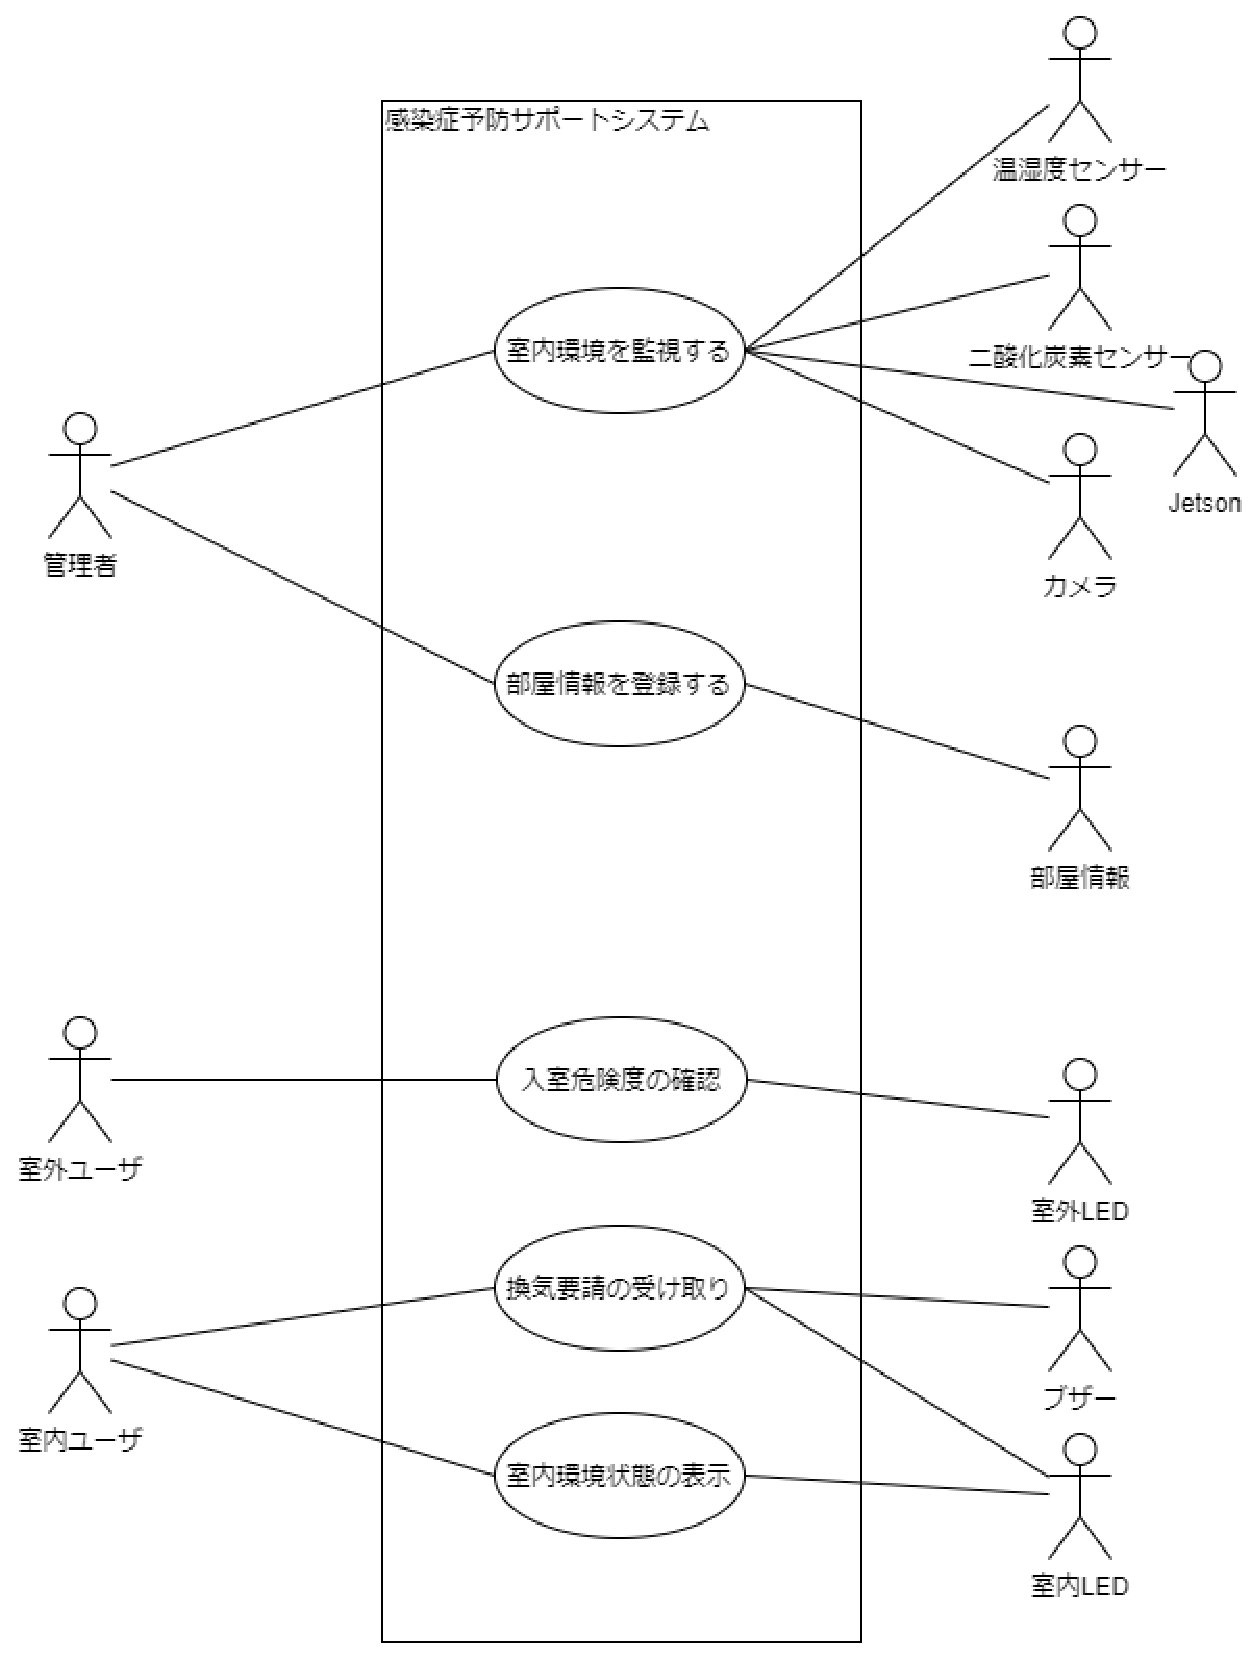
\includegraphics[width = 15cm]{./picture/usecase_3.eps}
\caption{ユースケース図}
\label{usecase}
\end{figure}

各ユースケースの詳細について述べる.
「室内状況を監視する」ユースケースは,管理者によって開始され,一定時間ごとに部屋状況の評価を行う.
具体的には,センサデバイスに接続された温湿度センサ,二酸化炭素センサとJetsonに接続されているWebカメラの画像をもとにJetsonが部屋状況の推定,評価を行う.
「部屋情報を登録する」ユースケースは,管理者によって開始され,システムに部屋情報を登録するものである.
この部屋情報は,学校や団体で指定されているガイドライン上で何人が上限であるかを計算するために,部屋の敷地面積をシステムに登録する.
「入室危険度の確認」ユースケースは,部屋の外にいる人が室外表示デバイスを介して部屋状況を確認するものである.
監視によって評価された部屋状況に応じて,部屋の入り口付近に設置した室外表示デバイスのLEDが点灯する.
点灯しているLEDの色を部屋の外にいる人が確認することで入室危険度を知ることができる.
「換気要請の受け取り」ユースケースは,屋内にいる人が換気が必要な状況であるかどうかを知るものである.
監視によって評価された部屋状況に応じ,換気が必要と判断された場合,室内にあるJetsonに接続されたLEDが点灯し,同時にブザーが鳴る.
これによって,システムから換気要請が出ていることを屋内にいる人が確認できる.
「室内環境状態の表示」ユースケースは,屋内にいる人が温湿度状態が危険な状態にあるかどうかを知るものである.
監視によって評価された部屋状況に応じ,特に温湿度が適正範囲内でなかった場合,室内にあるJetsonに接続されたLEDが点灯する.
これを受け,部屋の中にいる人はエアコンや加湿器等を適正に設定することを促され,感染症リスクが高くなりにくい環境に改善できる.

このうち,「室内状況を監視する」,「入室危険度の確認」,「換気要請の受け取り」,「室内環境状態の表示」を高重要な機能とした.
「部屋情報を登録する」ユースケースにおいては,本研究の目的においては必須なものではないため,重要度を低く設定した.
監視する機能の呼び出し時に,その都度入力を求めることでこれに替え,本研究においては開発対象外とすることにした.

本システムにおいては,部屋が使用されない時間がある程度存在するとしているため,夜間は監視の作業を一度止めることとした.
これにより,重要度の低い時にセンサの使用を止め,センサデバイスの連続動作可能時間の長時間化を図った.

上記の設計を受け,総合テストのテスト項目を表\ref{sougoutest_koumoku}の通り作成した.
\begin{table}[htbp]
    \centering
    \caption{総合テスト項目}
    \label{sougoutest_koumoku}
    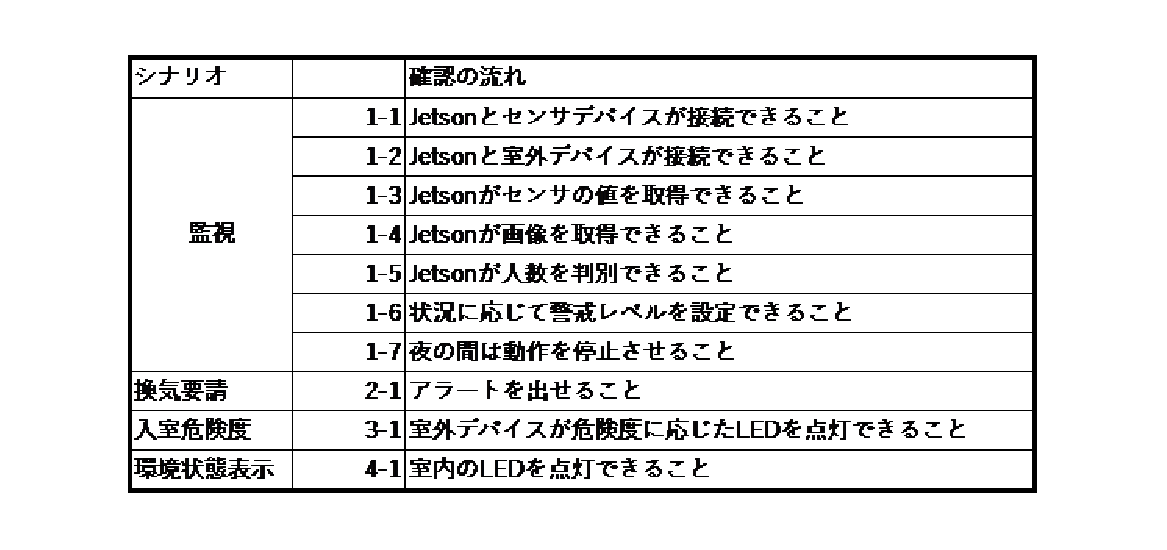
\includegraphics[width = 15cm]{./picture/sougoutest_koumoku.eps}
\end{table}

% スマートモビリティレジシステムがどのような機能をもって,どのように振る舞いをもつかを表すためにユースケース図を作成した.
% 以下に最初に作成した図\ref{usecase1}を載せる.

% \begin{figure}[htbp]
% \centering
% \includegraphics[width = 9cm]{./picture/usecase1.eps}
% \caption{ユースケース図(1)}
% \label{usecase1}
% \end{figure}


% 図\ref{usecase1}においてユースケースとしてはカゴの登録,商品をカゴに入れる,カゴを持って決済ゲートを通る,QRコードを読み取り決済するの4つとする.そこで,ユーザ登録から決済までの手順を簡単化するために,ユースケースを見直し,全体のユースケース数を削減する.

% %退店管理がどうなってたか思い出せないため,usecase2の図はお蔵入り予定
% %\begin{figure}[htbp]
% %\centering
% %\includegraphics[width = 11cm]{./picture/usecase2.eps}
% %\caption{ユースケース図(2)}
% %\label{usecase2}
% %\end{figure}

% 全体のユースケース数を削減したユースケース図を図\ref{usecase3}に示す.

% \begin{figure}[htbp]
% \centering
% \includegraphics[height = 9cm,width = 9cm]{./picture/usecase3.eps}
% \caption{ユースケース図(2)}
% \label{usecase3}
% \end{figure}


% 図\ref{usecase3}では,QRコードを読み取り決済する部分を,カゴの返却時にカゴの情報と顧客情報と結び付け,自動的に決済を行う仕様としたためユースケースが登録・買い物・決済の3つとなりより簡素化された.

% また,買い物の段階で商品情報をリアルタイムに収集・送信する必要があるため,カゴに取り付けられる小型サイズであり低価格かつ低消費電力のシングルボードコンピュータ(Raspberry Pi)を用いる.

% ユーザ登録と決済の方法に関しては,QRコードを用いる案と,ICタグを用いる案の2つを検討し,それぞれの案についてシナリオとユースケース図を作成し,後に優先度の高い範囲を切り出した.


% QRコードを用いた場合のスマートモビリティシステムのシナリオは下記の表\ref{sina_qr}のとおりである.


% \begin{table}[htb]
% \begin{center}
% \caption{QRコードを用いたシステムのシナリオ}
% \begin{tabular}{|l|c|} \hline
%  & シナリオ \\ \hline \hline
% 登録 & カゴのQRコードを顧客が読み取る \\
% 買い物 & 商品を置く→バーコード認識→商品DB追加・削除→結果通知 \\
% 決済 & カゴのQRコードを決済ゲートが読み取る→決済を行う \\ \hline
% \end{tabular}
% \label{sina_qr}
% \end{center}
% \end{table}

% また,QRコードを用いたスマートモビリティシステムのユースケース図を図\ref{usecase_qr}に示す.

% \begin{figure}[htbp]
% \centering
% \includegraphics[height = 9cm,width = 9cm]{./picture/usecase_qr.eps}
% \caption{QRコードを用いたシステムのユースケース図}
% \label{usecase_qr}
% \end{figure}

% 図\ref{usecase_qr}に示すように,まず,カゴにQRコードを印刷したものを貼りつける.QRコードには固有のカゴ情報が含まれており,ユーザが携帯電話等で読み取るとWebページへ遷移し顧客情報を入力する流れとなる.QRコードを入店時顧客が携帯電話等で読み取り,カゴ情報を顧客情報を結びつける.退店時は出口ゲートに設置したWebカメラでカゴのQRコードを読み取り,最終決済を行う.


% 次に,ICタグを用いた場合のスマートモビリティシステムのシナリオを下記の表\ref{sina_ic}へ,ユースケース図を図\ref{usecase_ic}に示す.


% \begin{table}[htb]
% \begin{center}
% \caption{ICタグを用いたシステムのシナリオ}
% \begin{tabular}{|l|c|} \hline
%  & シナリオ \\ \hline \hline
% 登録 & カゴのICタグをゲートが読み取る \\
% 買い物 & 商品を置く→バーコード認識→商品DB追加・削除→結果通知 \\
% 決済 & カゴのICタグをゲートが読み取る→決済を行う \\ \hline
% \end{tabular}
% \label{sina_ic}
% \end{center}
% \end{table}


% \begin{figure}[htbp]
% \centering
% \includegraphics[height = 9cm,width = 9cm]{./picture/usecase_ic.eps}
% \caption{ICタグを用いたシステムのユースケース図}
% \label{usecase_ic}
% \end{figure}

% 図\ref{usecase_ic}においては,カートもしくはカゴにICタグを取り付け,入退店時にリーダーを設置したゲートを通ることで,カゴ情報と顧客情報を管理する.

% %以下は3-2もしくは3-3で評価しようかな(下記の記述移動可能性)

% 以上の2つのユーザ登録と決済方法に対して,3.1節で述べたシステムへの要求事項を関して,下記の表\ref{test}で評価した.


% \begin{table}[htb]
% \begin{center}
% \caption{評価表}
% \begin{tabular}{|l||c|c|} \hline
%  & QRコード & ICタグ \\ \hline \hline
% 従来のセルフレジよりコストは抑えられるか & 〇 & × \\
% 既存の中小店でも導入が容易か & 〇 & △ \\
% 従来のセルフレジより簡単な動作で決済まで行えるか & × & 〇 \\ \hline
% \end{tabular}
% \label{test}
%   \end{center}
% \end{table}


% %具体的なカメラの台数やICタグの価格等を下記へ
% 評価結果より,QRコードを用いる案のほうがコストの面で優れている.しかしながら,簡単に決済まで行えるかという基準においては,携帯電話のカメラを起動して読み込む動作を顧客が行わなければならない点からQRコードを用いる案はあまり優れていないといえる.本研究では,以上の2つの登録決済方法ともにサポートできるスマートモビリティレジシステムを設計した.

% また,最終的に本研究で実装対象とした優先度の高い項目においてのシナリオ,およびユースケース図はそれぞれ下記の図\ref{use}と表\ref{sina}のとおりである.


% \begin{figure}[htbp]
% \centering
% \includegraphics[width = 9cm]{./picture/usecase_saishu.eps}
% \caption{高優先度のシステムのユースケース図}
% \label{use}
% \end{figure}

% \begin{table}[htbp]
% \begin{center}
% \caption{高優先度のシステムのシナリオ}
% \begin{tabular}{|l|c|} \hline
%  & シナリオ \\ \hline \hline
% 買い物 & 商品を置く→バーコード認識→商品DB追加・削除→結果通知 \\
% 決済 & 決済を行う \\ \hline
% \end{tabular}
% \label{sina}
% \end{center}
% \end{table}

% なお,優先度の高い項目において,総合テストの際に用いて,各実装対象のシナリオに基づいたテスト項目を下記の表\ref{sogo}に示す.

% \begin{table}[htbp]
% \centering
% \caption{総合テスト項目}
% 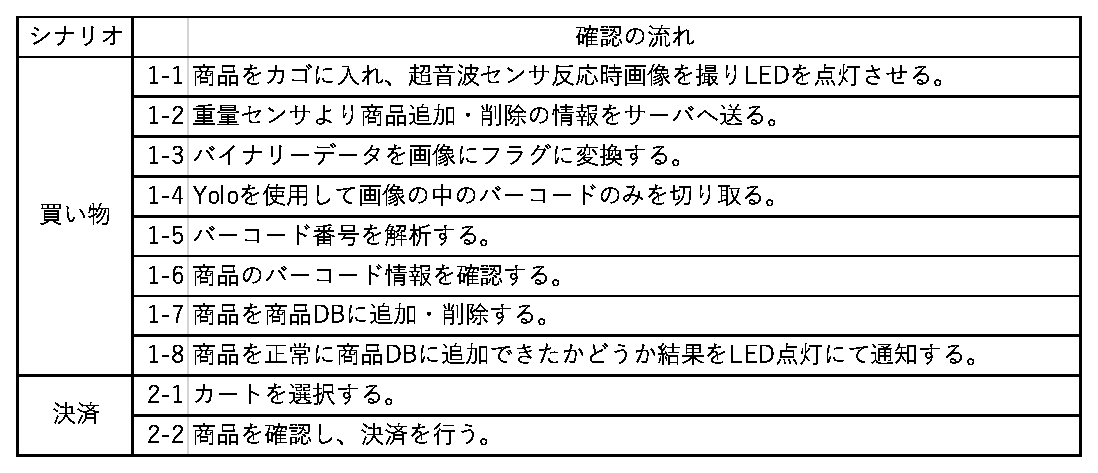
\includegraphics[width = 15cm]{./picture/sogo.eps}
% \label{sogo}
% \end{table}

%\newpage